\begin{problem}{우물}
	{standard input}{standard output}
	{3 seconds}{64 megabytes}{}
	
	
	범수는 지구이웨의 사막을 가로지르는 카제비 호수를 따라 여행을 다니고 있다. 불행하게도, 카제비호수가 말라버려서 범수가 마실 물이 없어졌다. 그의 유일한 희망은 강바닥을 충분히 깊게 파 지하수가 샘솟는 우물을 만드는 것이다.

	범수는 자신의 상황을 잘 알기 때문에, 실제로 삽질을 시작하기 전에 모든걸 계획하려고 한다. 가장 큰 위협은 물이 나오는 수위에 도달하기 전에 범수가 힘을 다 써버리는 것이다. 그럴 경우 범수의 목숨이 위험하다. 범수는 힘이 다하기 전에 얼마나 삽질을 할 수 있는지를 알 수 있다. 그의 유일한 걱정은 산사태가 생길 가능성이 있다는 것이다. 그는 강바닥의 지형도를 당신에게 위성전화로 보내서, 삽질의 기울기가 최대한 완만하게 팔 수 있는 위치를 알려달라고 했다. 범수를 도와주자!
 
	\InputFile
	
	 첫째 줄에는 두 개의 정수 $n$과 $m$이 공백 하나로 구분되어 주어진다. ($1 \le n \le 1,000,000$, $1 \le m \le 10^{18}$) 두번째 줄에는 공백 하나로 구분된 $n$개의 정수 $x_1 , x_2 , \cdots, x_n$ ($1 \le x_i \le 10^9$)가 주어진다.
	 
	 범수는 $m$번 삽질을 하기 충분한 힘을 가지고 있다. $x_1, x_2, \cdots, x_n$은 카제비 호수의 강바닥의 지형도를 나타낸다. 이 수들은 물이 나올 때 까지 쌓인 모래의 양을 미터단위로 나타낸다. 삽질을 한번 하면 땅바닥의 모래의 양 즉, $x_i$가 1 줄어든다. 어떤 하나의 수 즉, $x_k$가 0이 된다면 범수는 물을 마실 수 있따는 것을 의미한다. 하지만 범수의 두번째 목표는 모래의 기울기를 나타내는 $z$를 최소화 하는 것이다.:

\begin{center}
	\Large
	$z =  \underset{i=1, 2, \cdots, n-1}{\max} |x_i - x_{i+1}|$
\end{center}

	답을 의미하는 $k$가 여럿 있다면, 아무것이나 출력해도 된다. $1, 2, \cdots, n$번 위치를 제외하고는 삽질을 하기 적당하지 않은 곳이다. -- 모래 대신에 바위가 있다. 범수가 삽질을 제한된 횟수 이내로 해서 물을 마실 수 있음은 보장된다.

	\OutputFile
	
	프로그램은 첫째 줄에 공백 하나로 구분된 두 정수를 출력해야 한다. 첫째 수는 범수가 물이 나올 때 까지 삽질을 해야하는 위치은 $k$이고, 둘째 수는 $z$의 최솟값이다.
	
	
	\SubtaskWithCost{1}{35}
	\begin{itemize}
		\item $n \le 10,000$
	\end{itemize}
	
	\SubtaskWithCost{2}{65}
	
	추가 제한조건이 없다.
	
	\Examples
		
	\begin{example}
	\exmp{
16 15
8 7 6 5 5 5 5 5 6 6 7 8 9 7 5 5
	}{%
1 2
	}%
	\end{example}
	
	\Note
	
	\begin{center}
	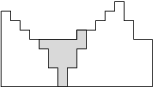
\includegraphics[]{stu.png}
	\end{center}
	
	위의 그림에서 범수가 할 수 있는 삽질이 회색으로 표시되어 있다.
	
        
\end{problem}

